\chapter{Résultats, Tests et Réalisations}

Ce chapitre est consacré à la présentation des résultats obtenus suite au développement de la plateforme. Il expose d'abord les réalisations visuelles de l'interface utilisateur, puis détaille de manière exhaustive les résultats des tests de validation de l'algorithme d'intelligence artificielle et du backend.

\section{Réalisations Visuelles (UI/UX)}

L'interface utilisateur est le point d'interaction critique. Elle doit retranscrire la complexité mathématique des algorithmes en visuels clairs et actionnables.

\subsection{La Charte ``Minimalist Blue''}
Nous avons configuré Ant Design via un \texttt{ConfigProvider} pour écraser le style par défaut et injecter notre propre identité visuelle. La couleur \textit{Navy} (\texttt{\#0f172a}) sert de base pour la structure (Menu, Header), garantissant un fort contraste, tandis que la couleur d'accentuation \textit{Teal} (\texttt{\#14b8a6}) guide l'œil de l'utilisateur vers les actions prédictives.

\subsection{Interfaces d'Authentification}
Afin de sécuriser l'accès aux prédictions, nous avons développé des interfaces de connexion et d'inscription épurées. Elles s'intègrent parfaitement dans le thème sombre de l'application et communiquent avec l'API Django pour générer et valider les jetons de sécurité JWT.

\begin{figure}[H]
    \centering
    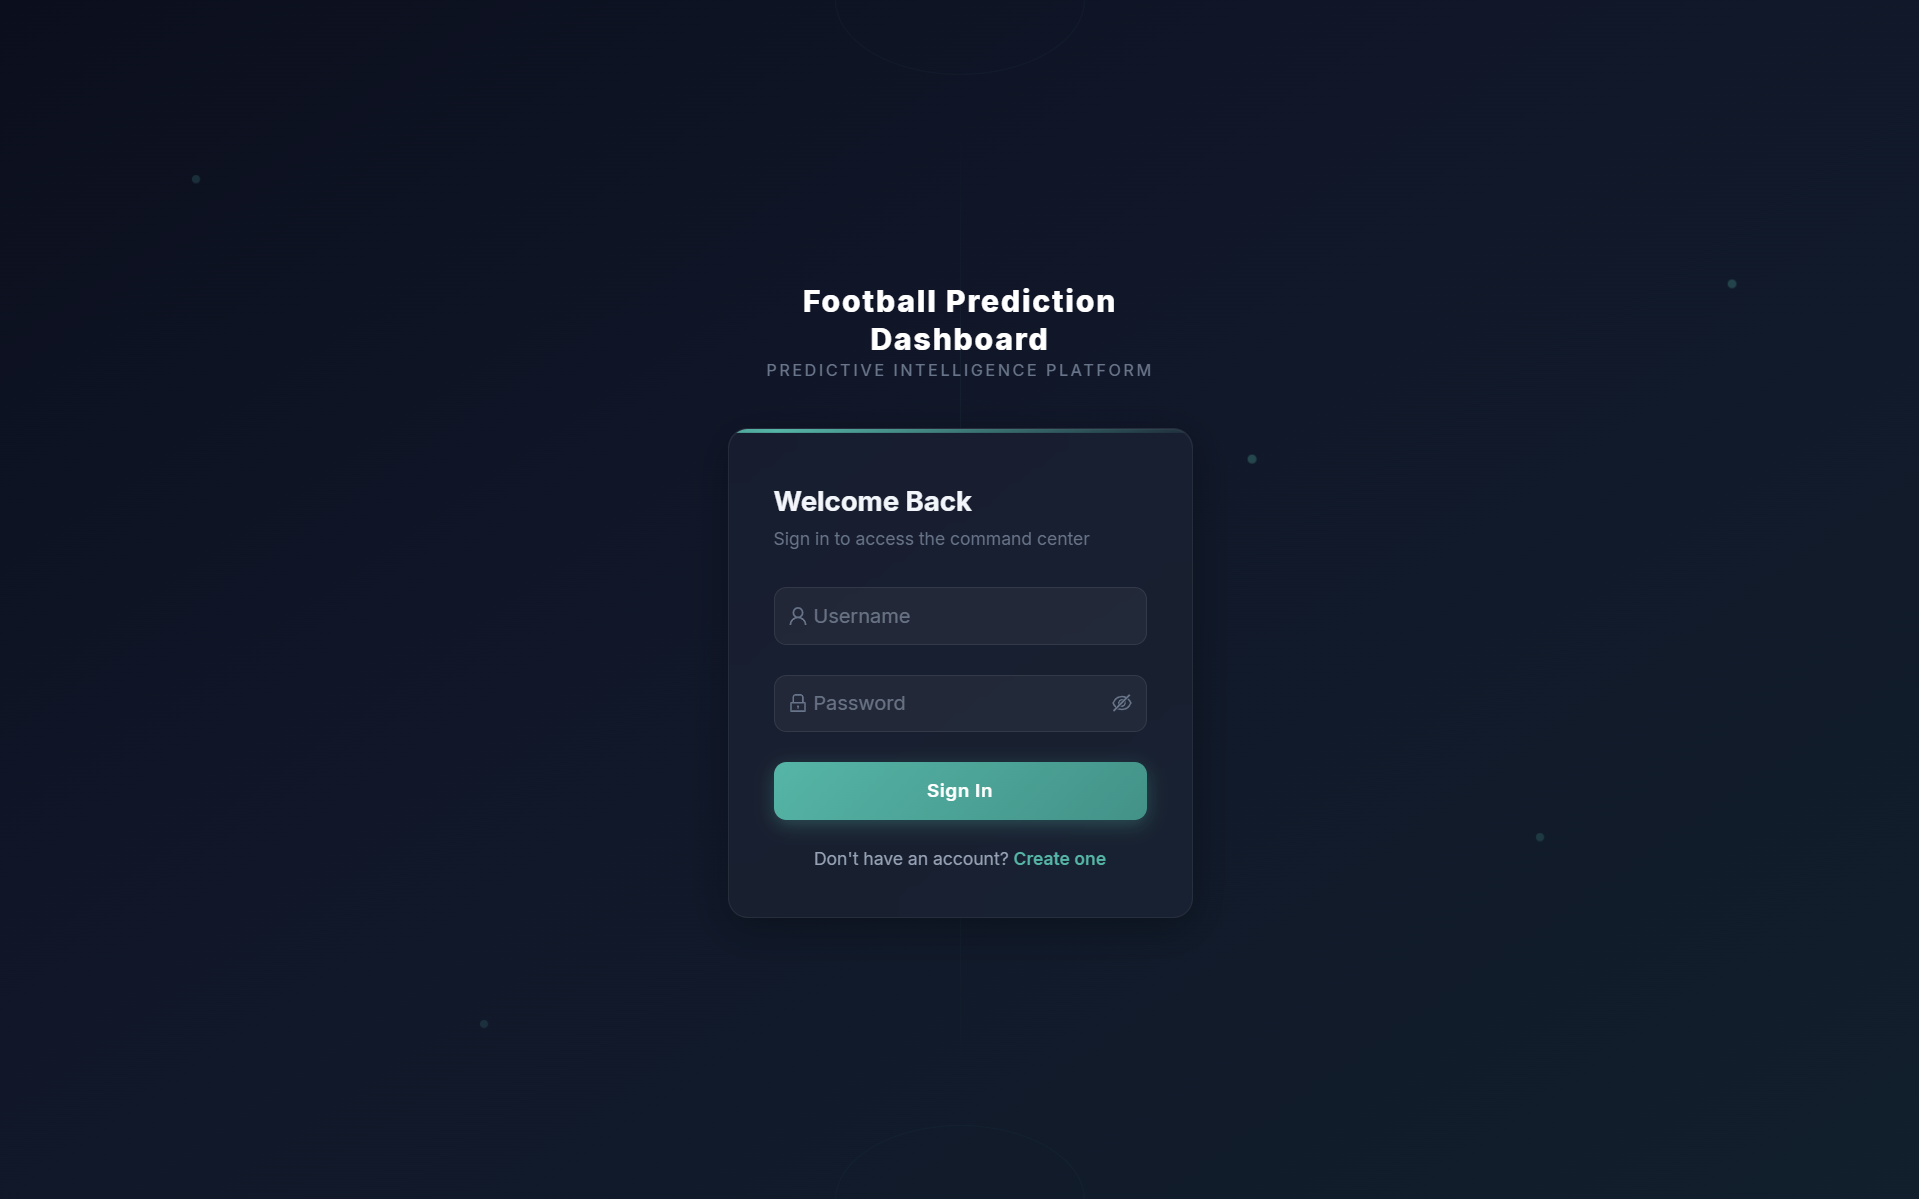
\includegraphics[width=0.85\textwidth]{logos/login.png}
    \caption{Interface de connexion (Sign In)}
\end{figure}

\begin{figure}[H]
    \centering
    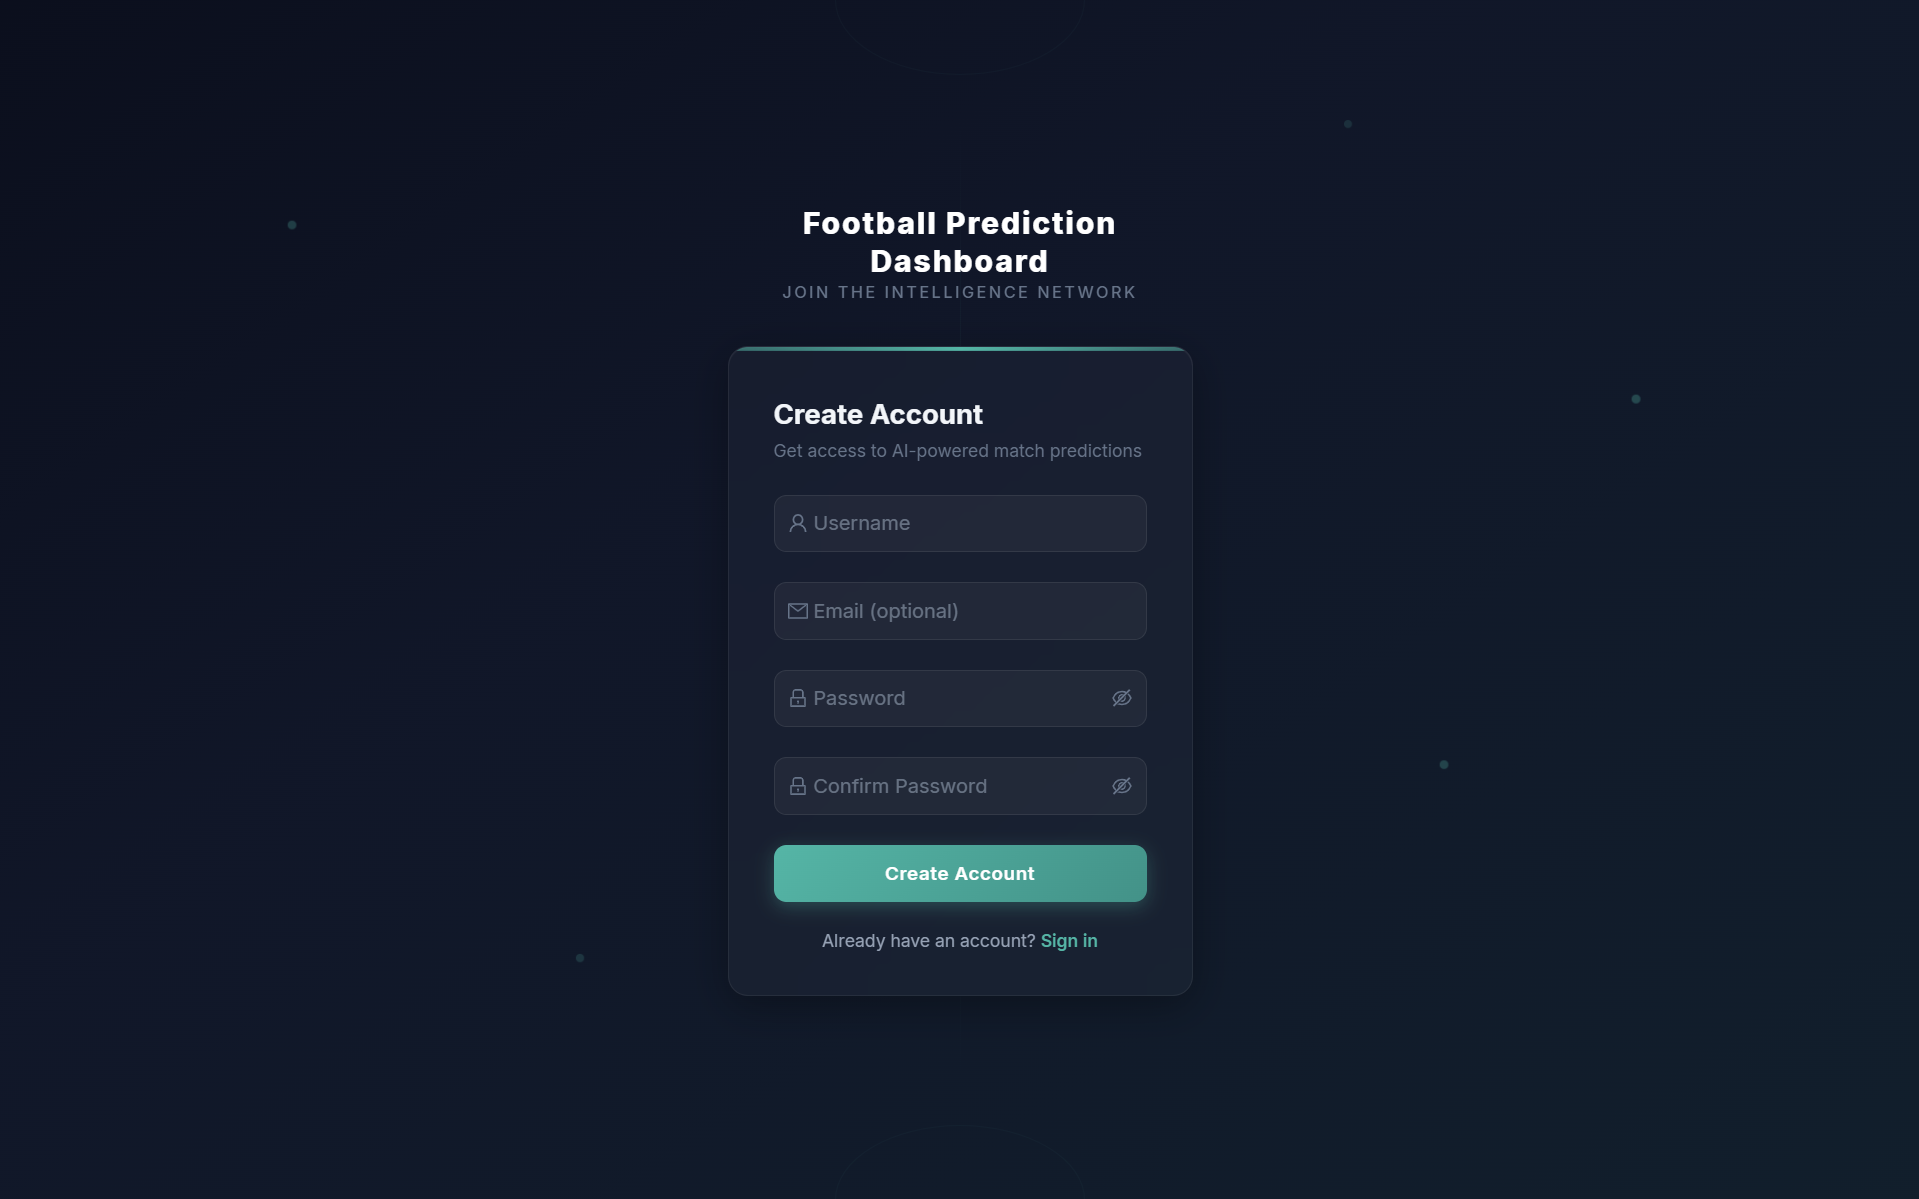
\includegraphics[width=0.85\textwidth]{logos/register.png}
    \caption{Interface de création de compte (Register)}
\end{figure}

\subsection{Panneau d'Administration}
Un espace réservé aux administrateurs a été mis en place pour la gestion de la plateforme. Ce panneau de contrôle (\textit{Admin Control Panel}) permet de visualiser la liste des utilisateurs inscrits et d'identifier rapidement leurs rôles (USER, ADMIN) au sein de l'application.

\begin{figure}[H]
    \centering
    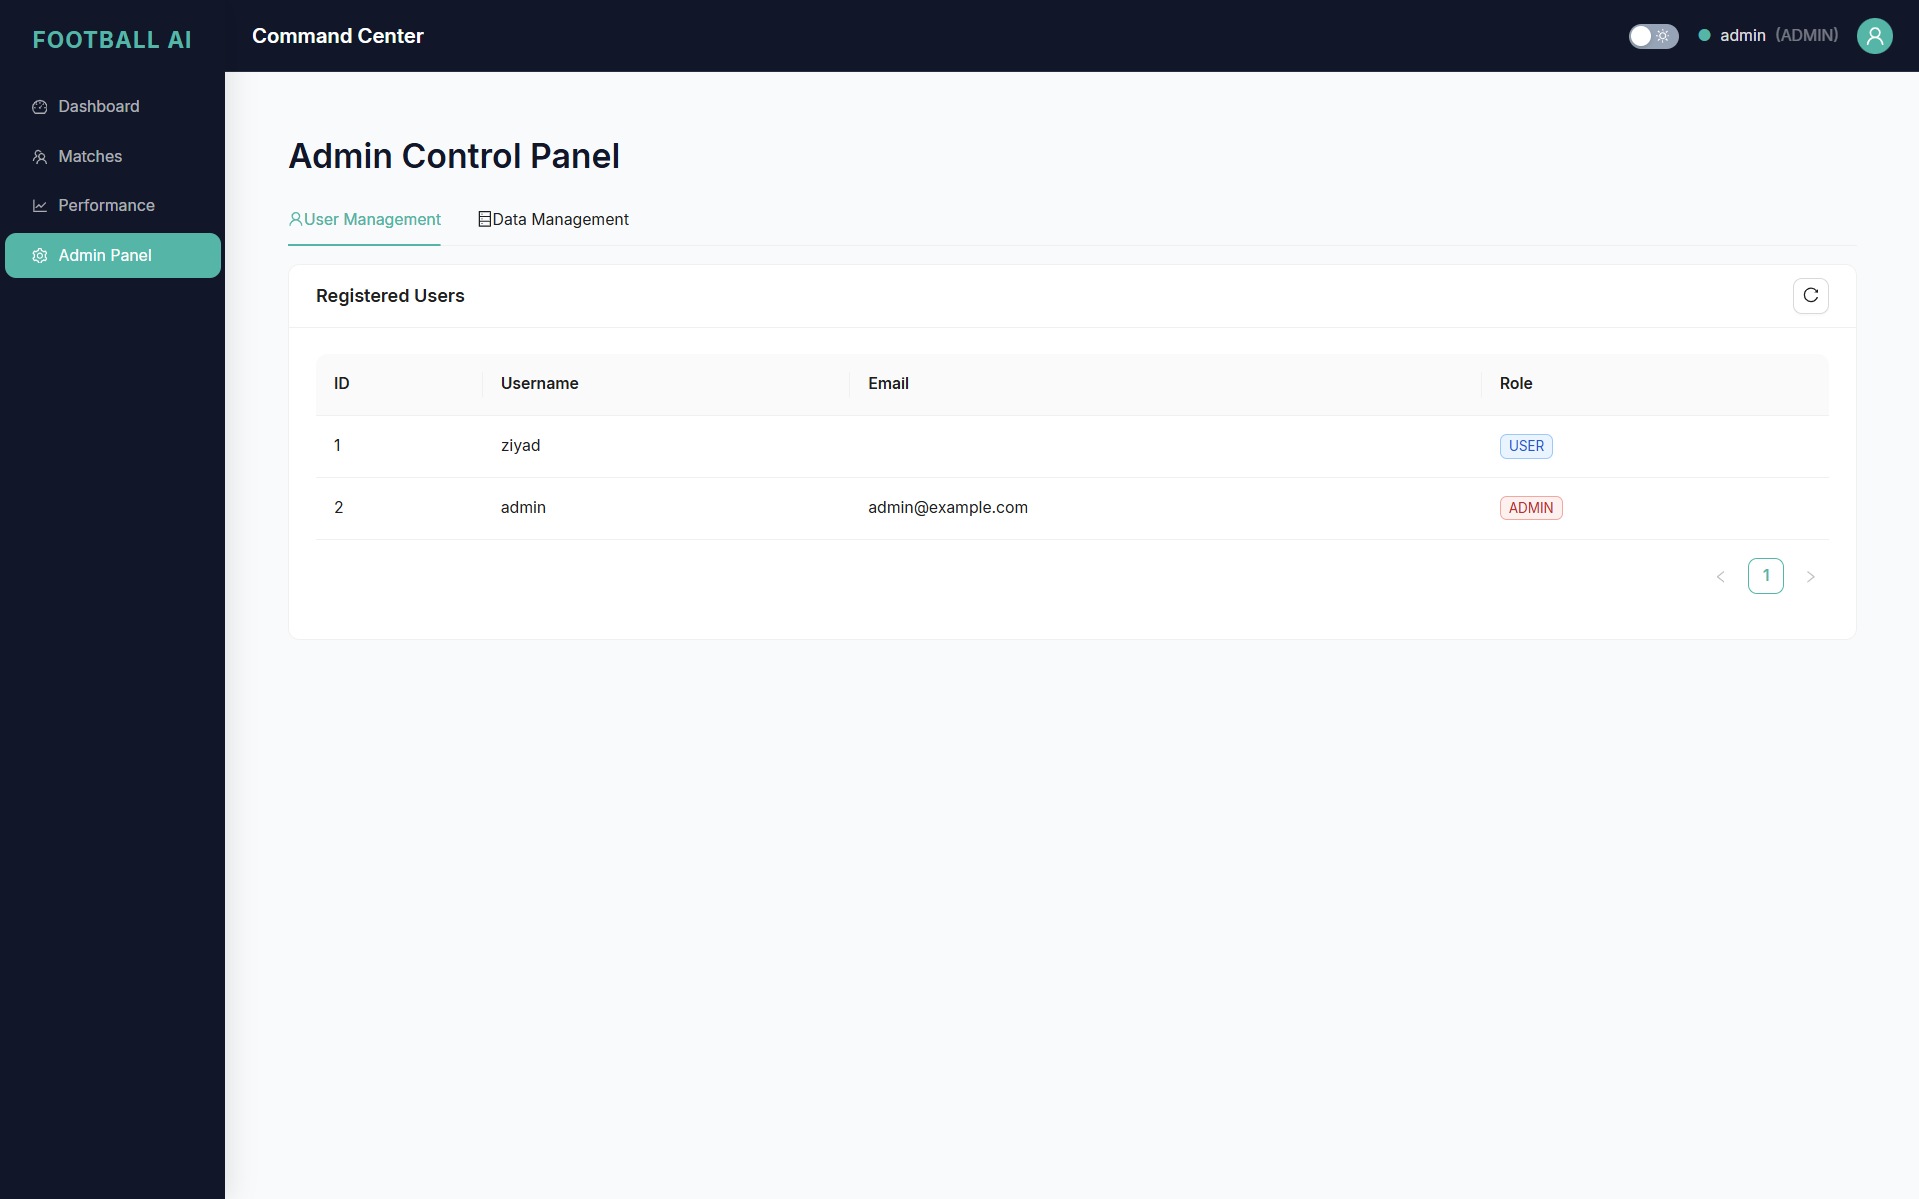
\includegraphics[width=0.95\textwidth]{logos/admin_panel.png}
    \caption{Interface de gestion des utilisateurs}
\end{figure}

\subsection{Le Centre de Commande et d'Analyse (Dashboard)}
Le composant central de l'application est le tableau de bord interactif (\textit{Command Center}). Il est organisé pour offrir une vision synthétique et détaillée des prédictions :
\begin{itemize}
    \item \textbf{Sélecteur de cible} : Permet de rechercher et de cibler un match spécifique.
    \item \textbf{Métriques clés} : Affiche instantanément la confiance de l'IA (ex: 75.64\%) et la précision globale du système (ex: 69.6\%).
    \item \textbf{Scorecard prédictive} : Présente la prédiction principale (ex: Match Nul) confrontée au résultat réel du terrain (ex: 2-2), validant visuellement la performance du modèle.
\end{itemize}

\begin{figure}[H]
    \centering
    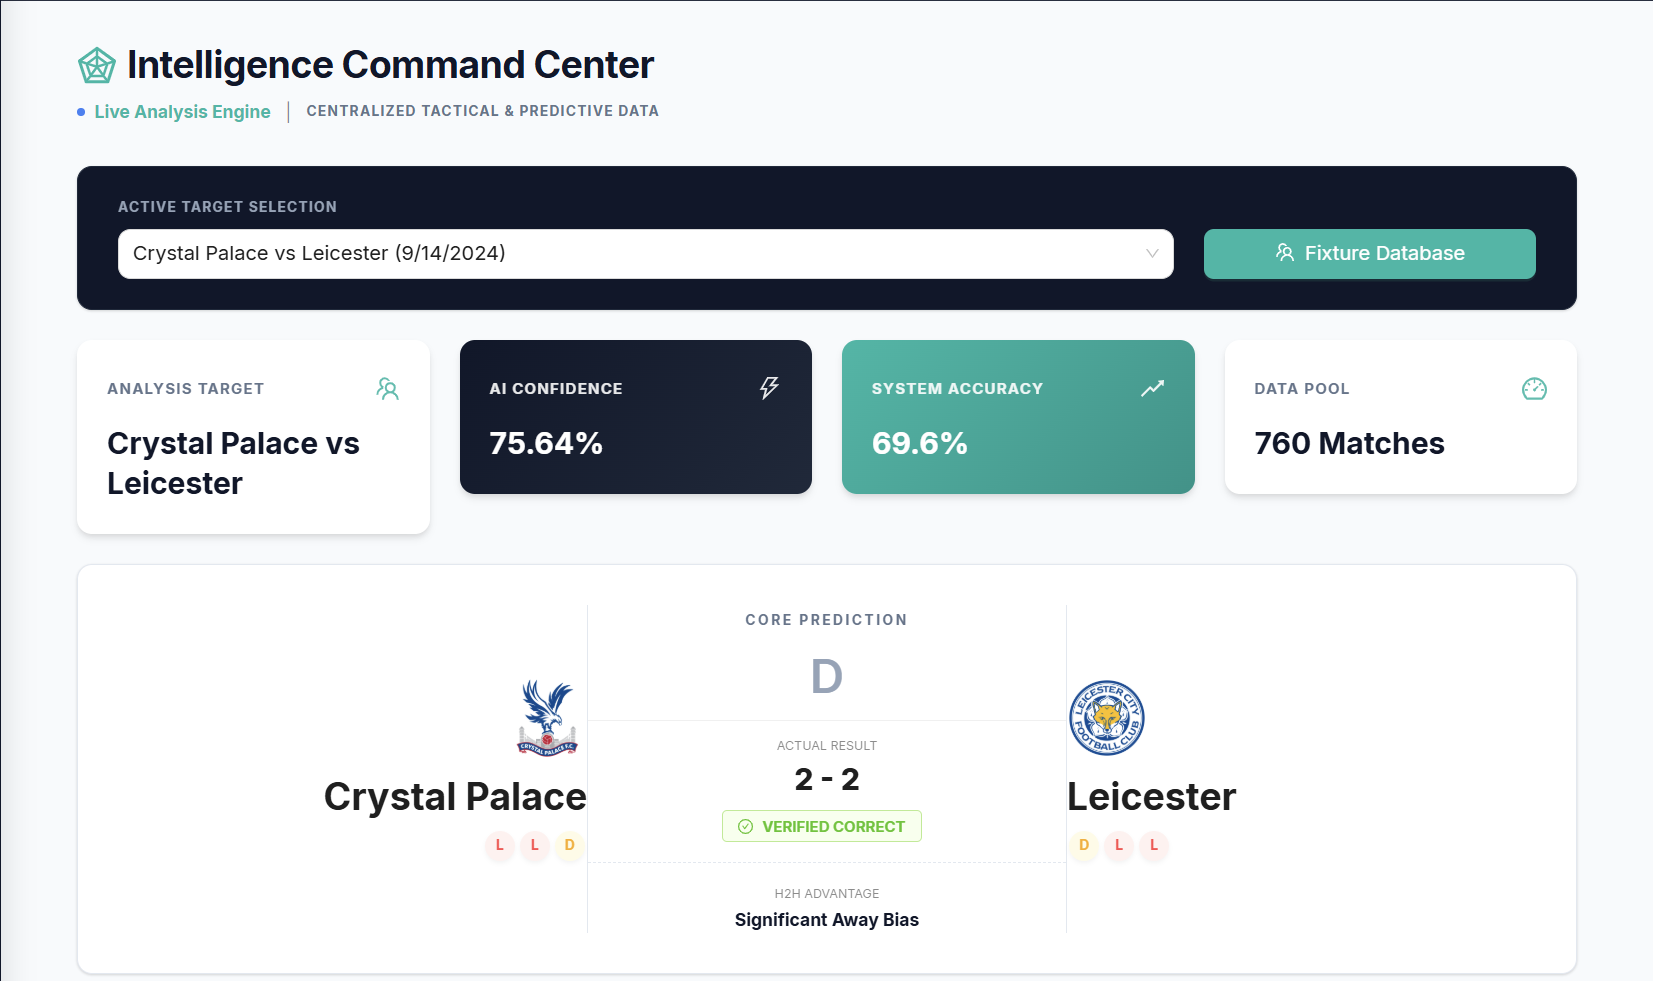
\includegraphics[width=0.95\textwidth]{logos/dashboard.png}
    \caption{Le centre de commande analytique interactif (Dashboard)}
\end{figure}

\subsection{Détails Analytiques et Tactiques}
Au-delà de la prédiction brute, le tableau de bord intègre une série de visualisations interactives permettant aux analystes de comprendre le raisonnement de l'intelligence artificielle et de comparer les dynamiques des deux équipes.

\begin{figure}[H]
    \centering
    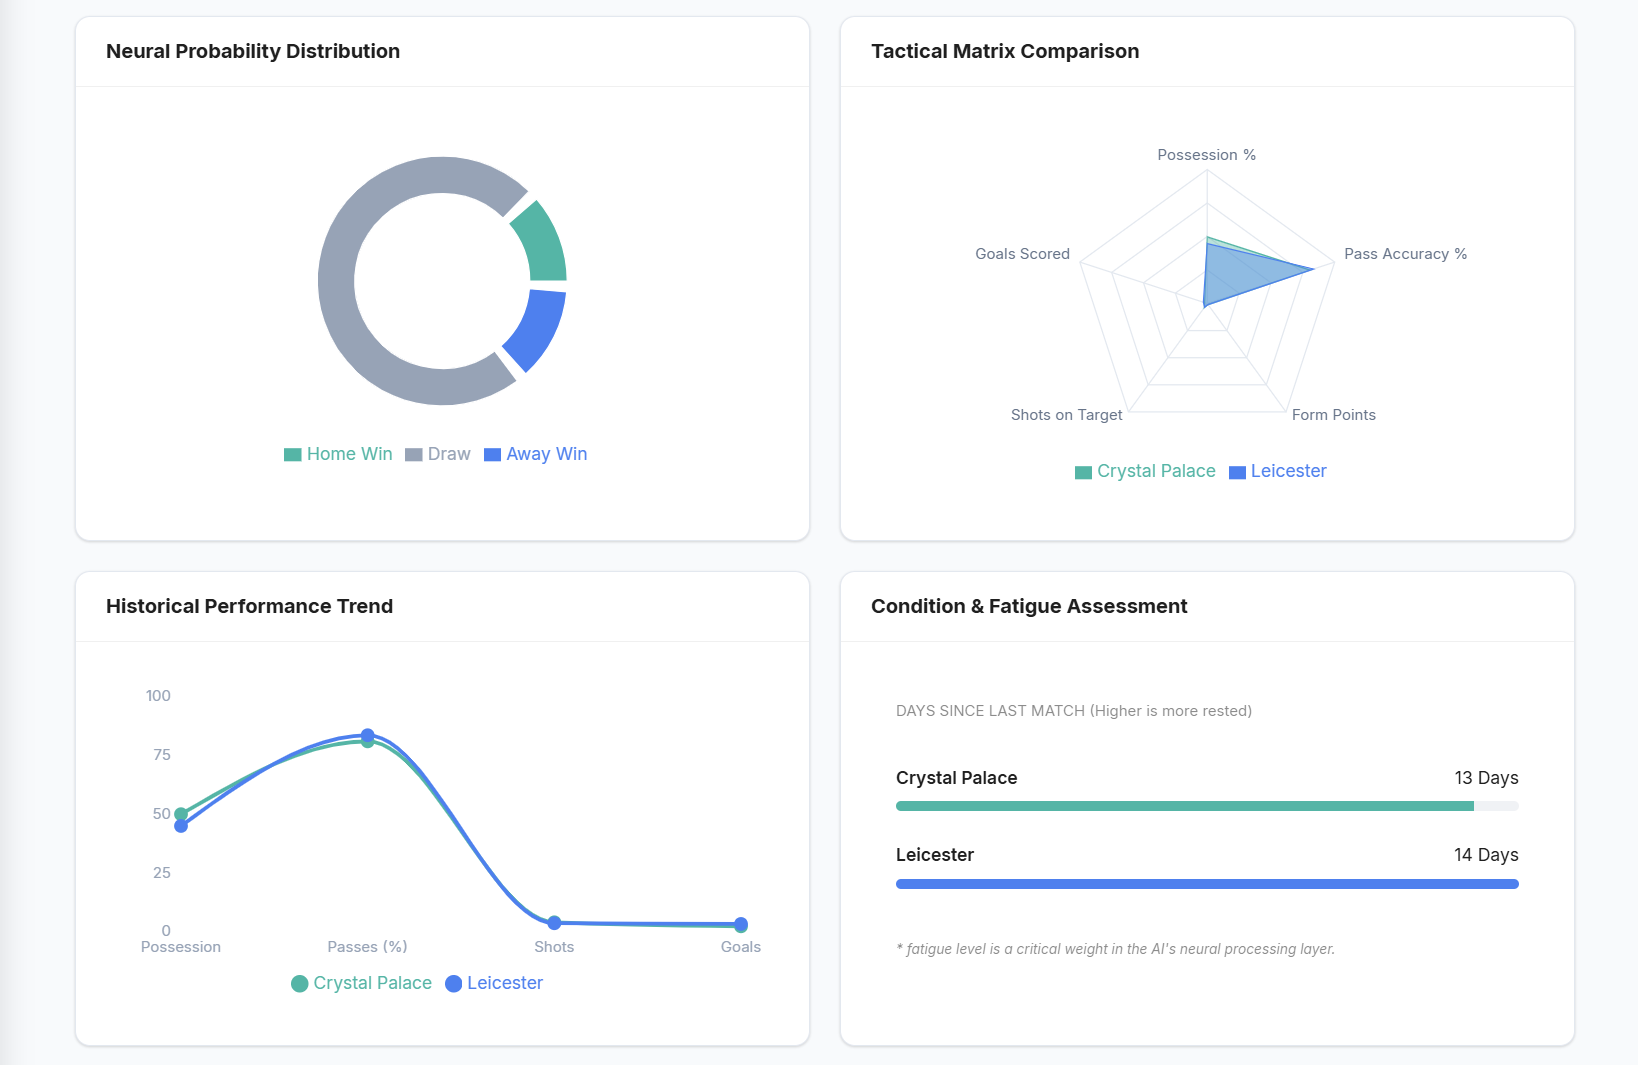
\includegraphics[width=0.95\textwidth]{logos/dashboard_metrics.png}
    \caption{Distribution probabiliste et comparaison sous forme de radar tactique}
\end{figure}

Les métriques stratégiques (Possession, Passes, Tirs) sont également confrontées directement à travers des graphiques en barres clairs, facilitant l'identification des forces en présence.

\begin{figure}[H]
    \centering
    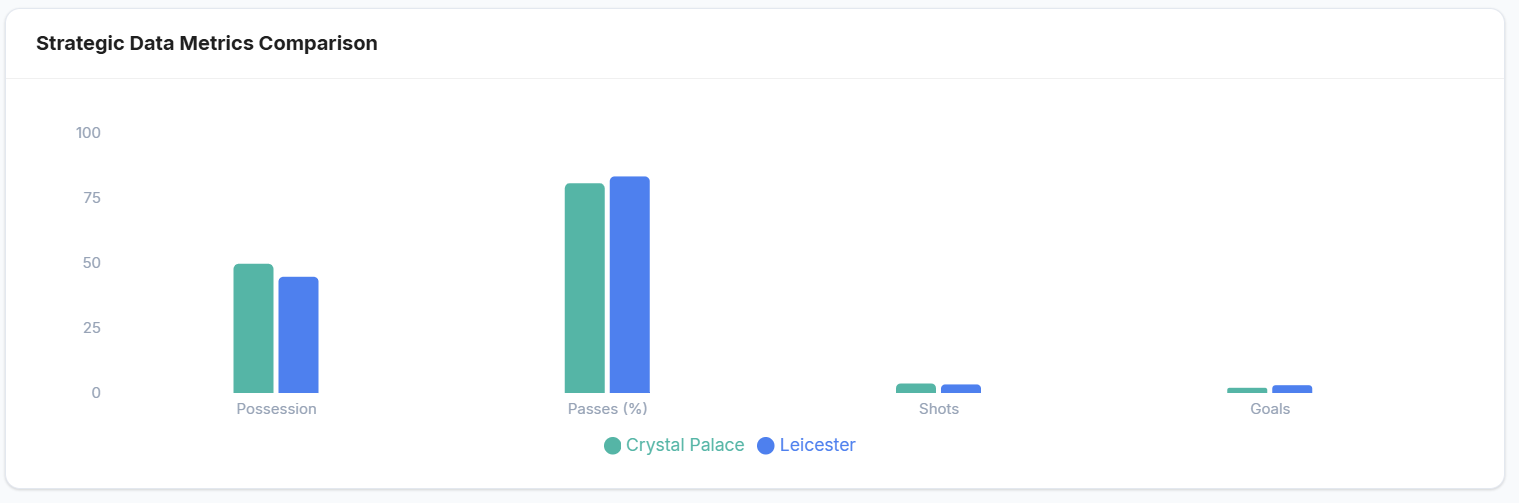
\includegraphics[width=0.95\textwidth]{logos/strategic_comparison.png}
    \caption{Comparaison des métriques de jeu de chaque équipe}
\end{figure}

Pour une vision de terrain, l'interface génère dynamiquement un rendu visuel de la composition tactique attendue (\textit{Tactical Pitch}), permettant de visualiser le positionnement spatial des joueurs (ex: 4-2-3-1). 

\begin{figure}[H]
    \centering
    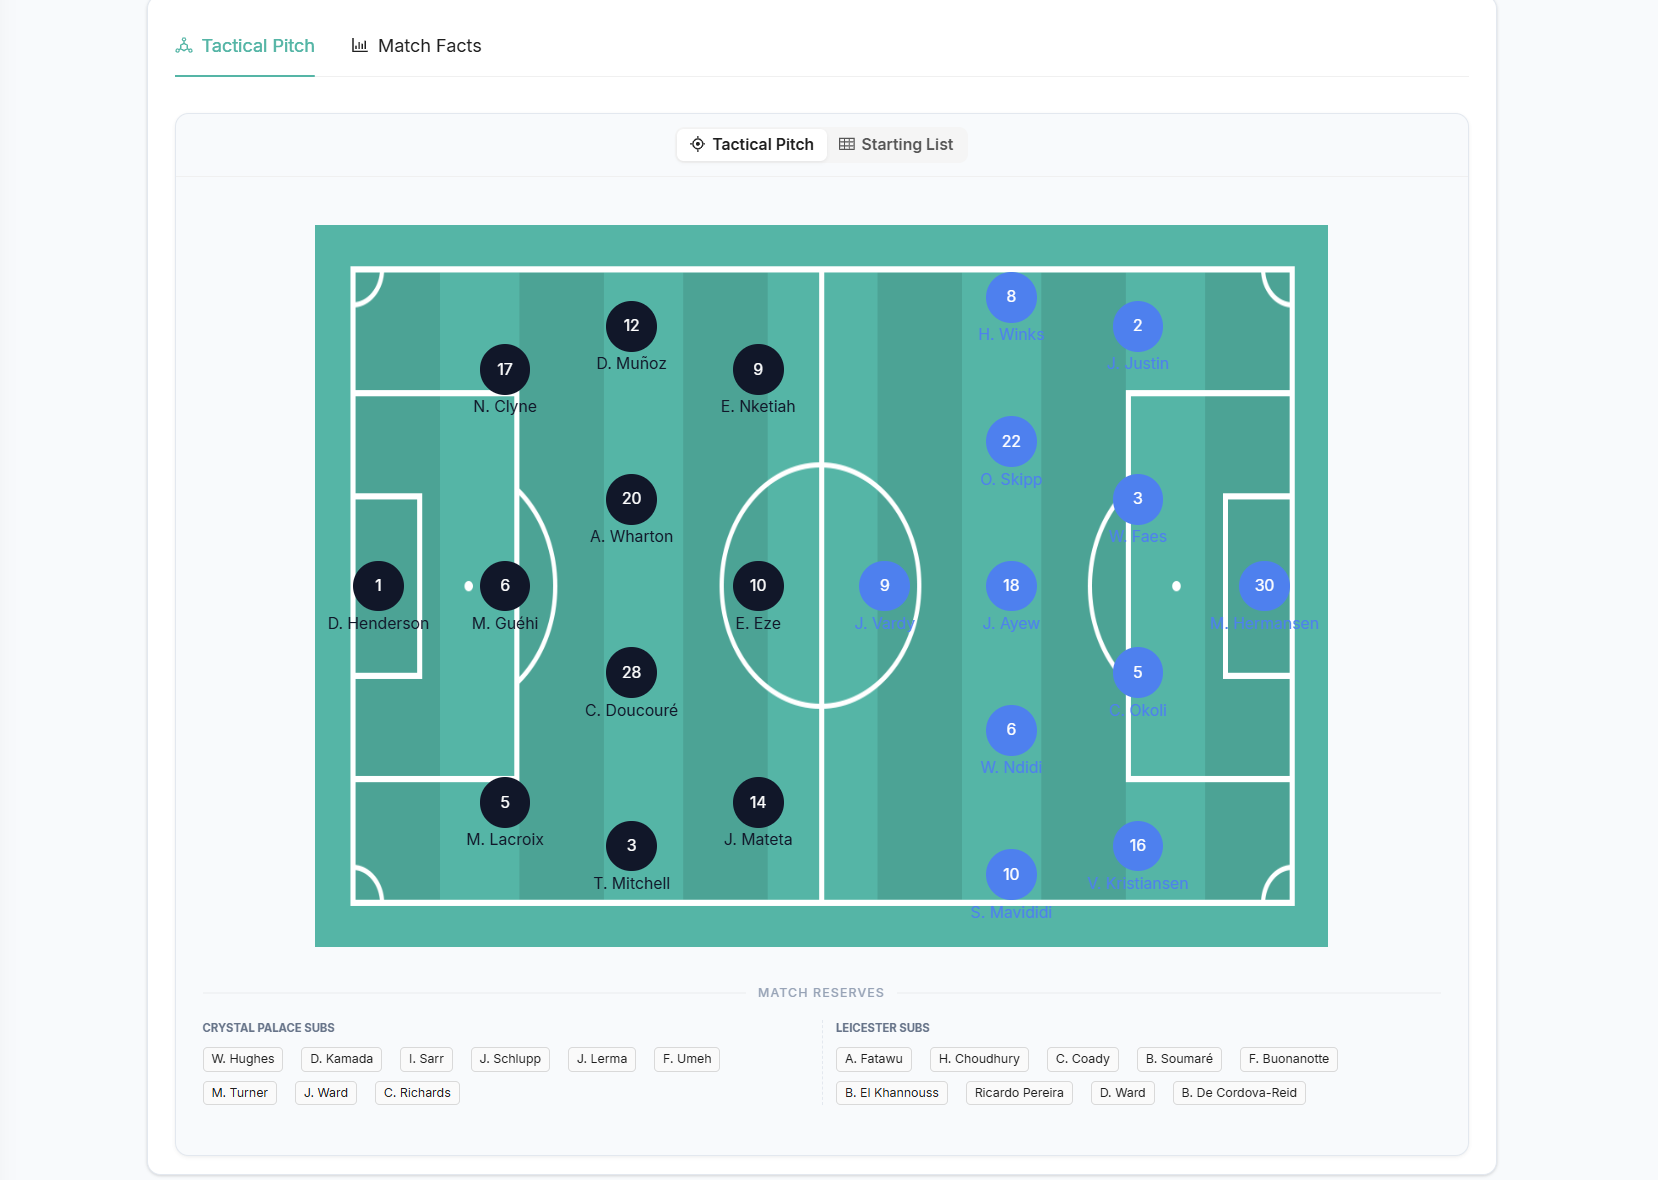
\includegraphics[width=0.95\textwidth]{logos/tactical_pitch.png}
    \caption{Rendu dynamique du terrain et composition des équipes}
\end{figure}

Enfin, un résumé global des faits du match (\textit{Match Facts}) jauge la domination globale entre l'équipe à domicile et celle à l'extérieur.

\begin{figure}[H]
    \centering
    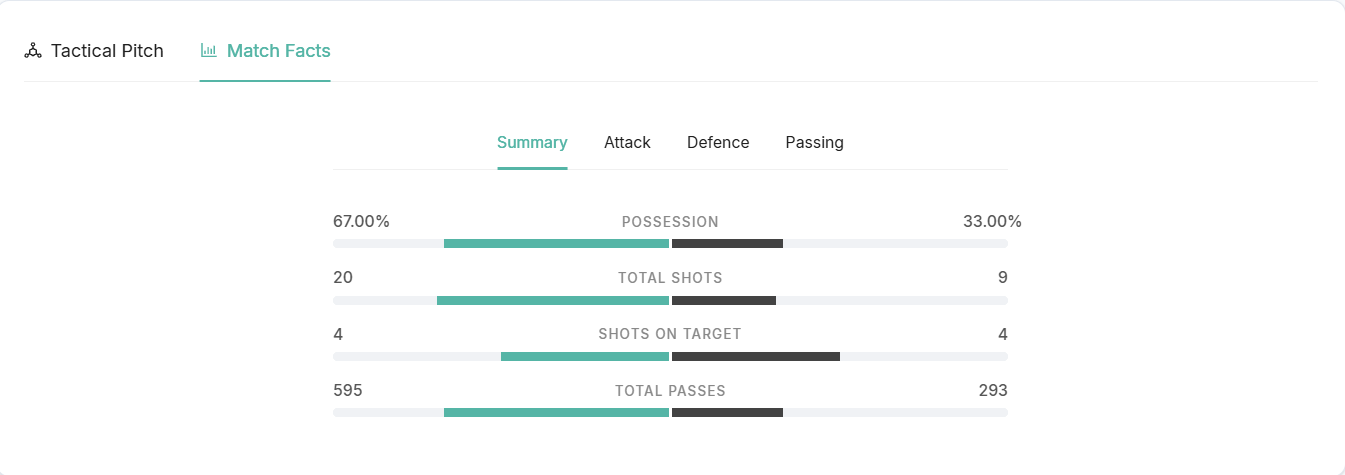
\includegraphics[width=0.95\textwidth]{logos/match_facts.png}
    \caption{Résumé statistique des dynamiques du match}
\end{figure}

\subsection{Exploration des Données et Historique}
Pour garantir une transparence totale vis-à-vis des utilisateurs, l'application intègre des vues dédiées à l'exploration des données brutes et à l'historique des performances.

\begin{figure}[H]
    \centering
    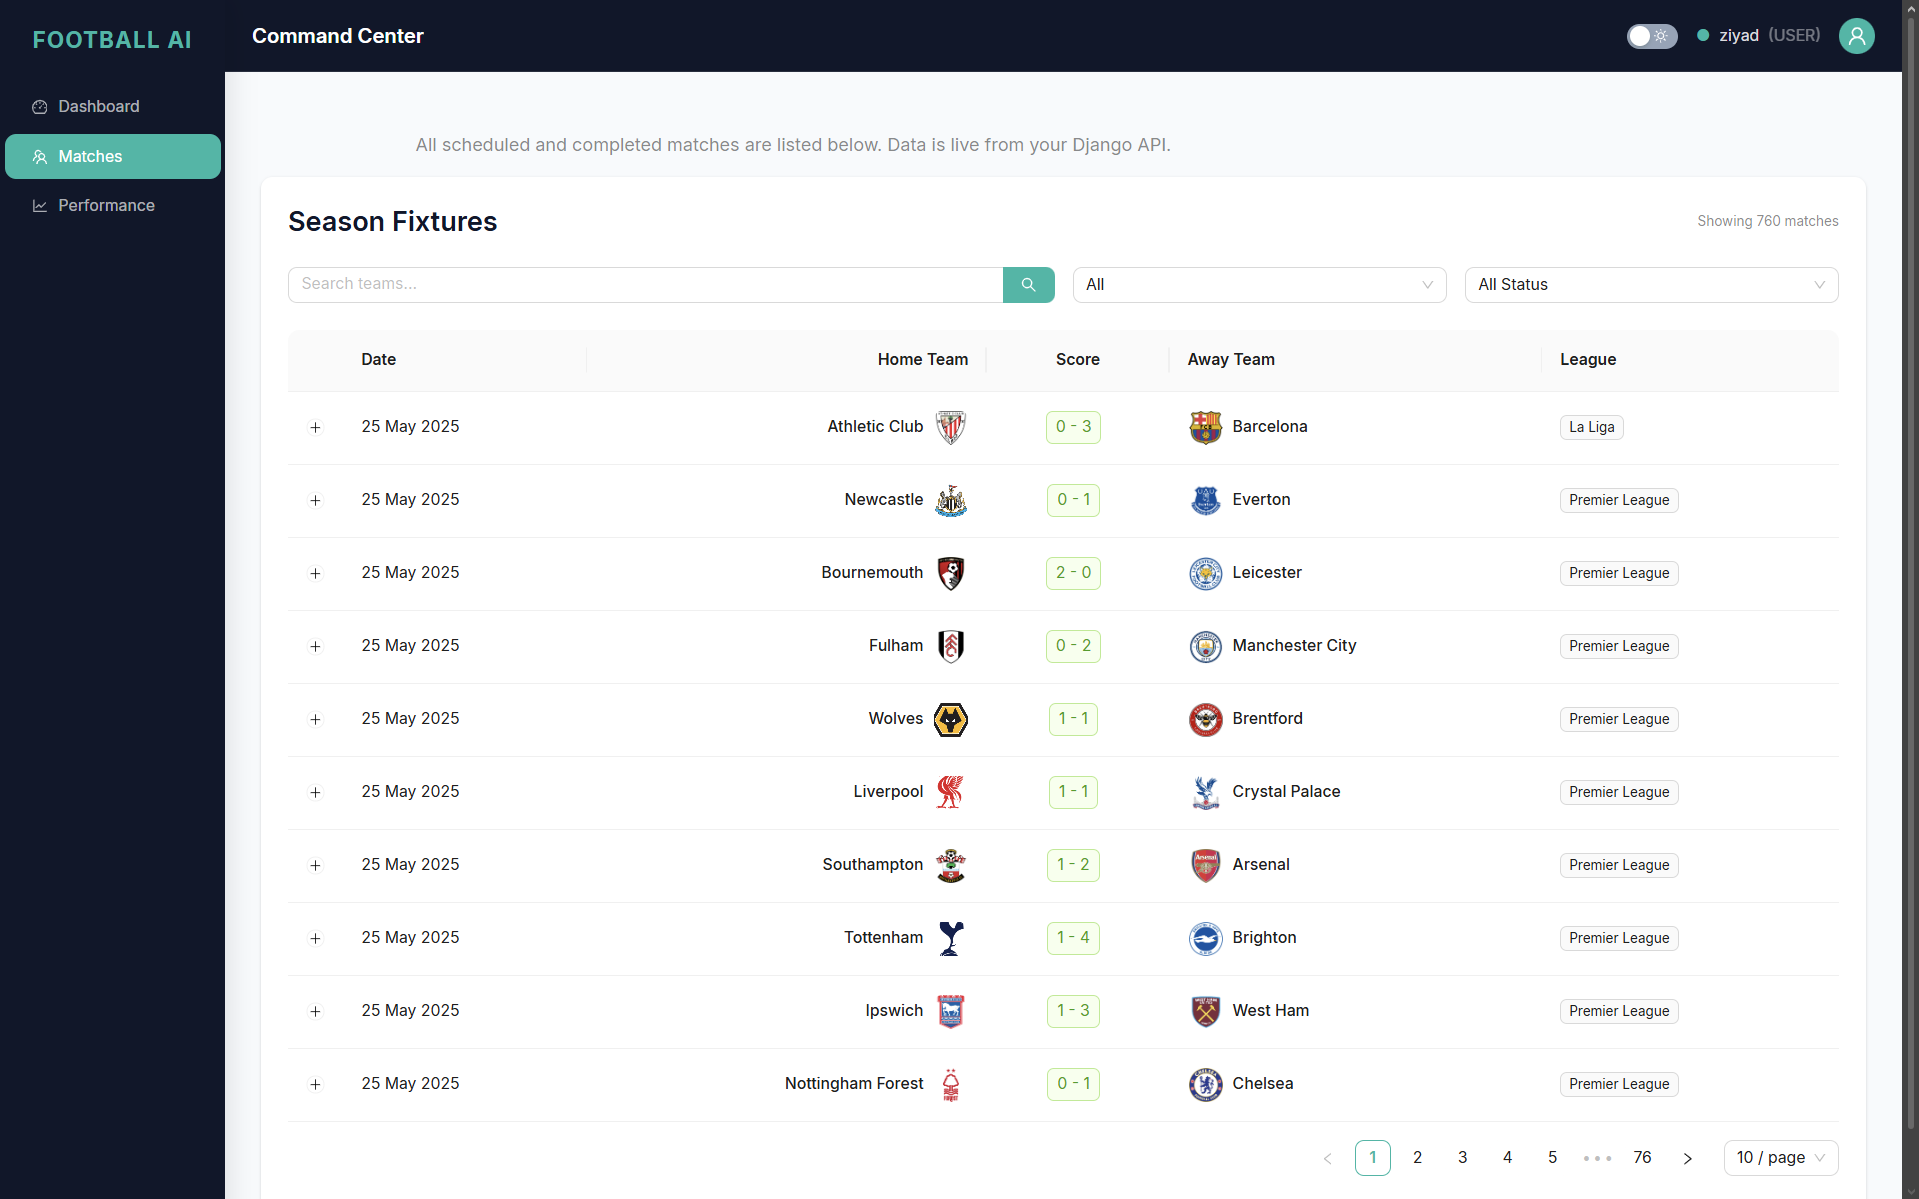
\includegraphics[width=0.95\textwidth]{logos/matches.png}
    \caption{Liste paginée des rencontres sportives synchronisées avec l'API}
\end{figure}

L'écran des performances dresse un bilan honnête des capacités du modèle, affichant un journal détaillé (\textit{Log}) comparant chaque prédiction de l'IA avec le résultat réel, permettant ainsi d'auditer l'intelligence artificielle en temps réel.

\begin{figure}[H]
    \centering
    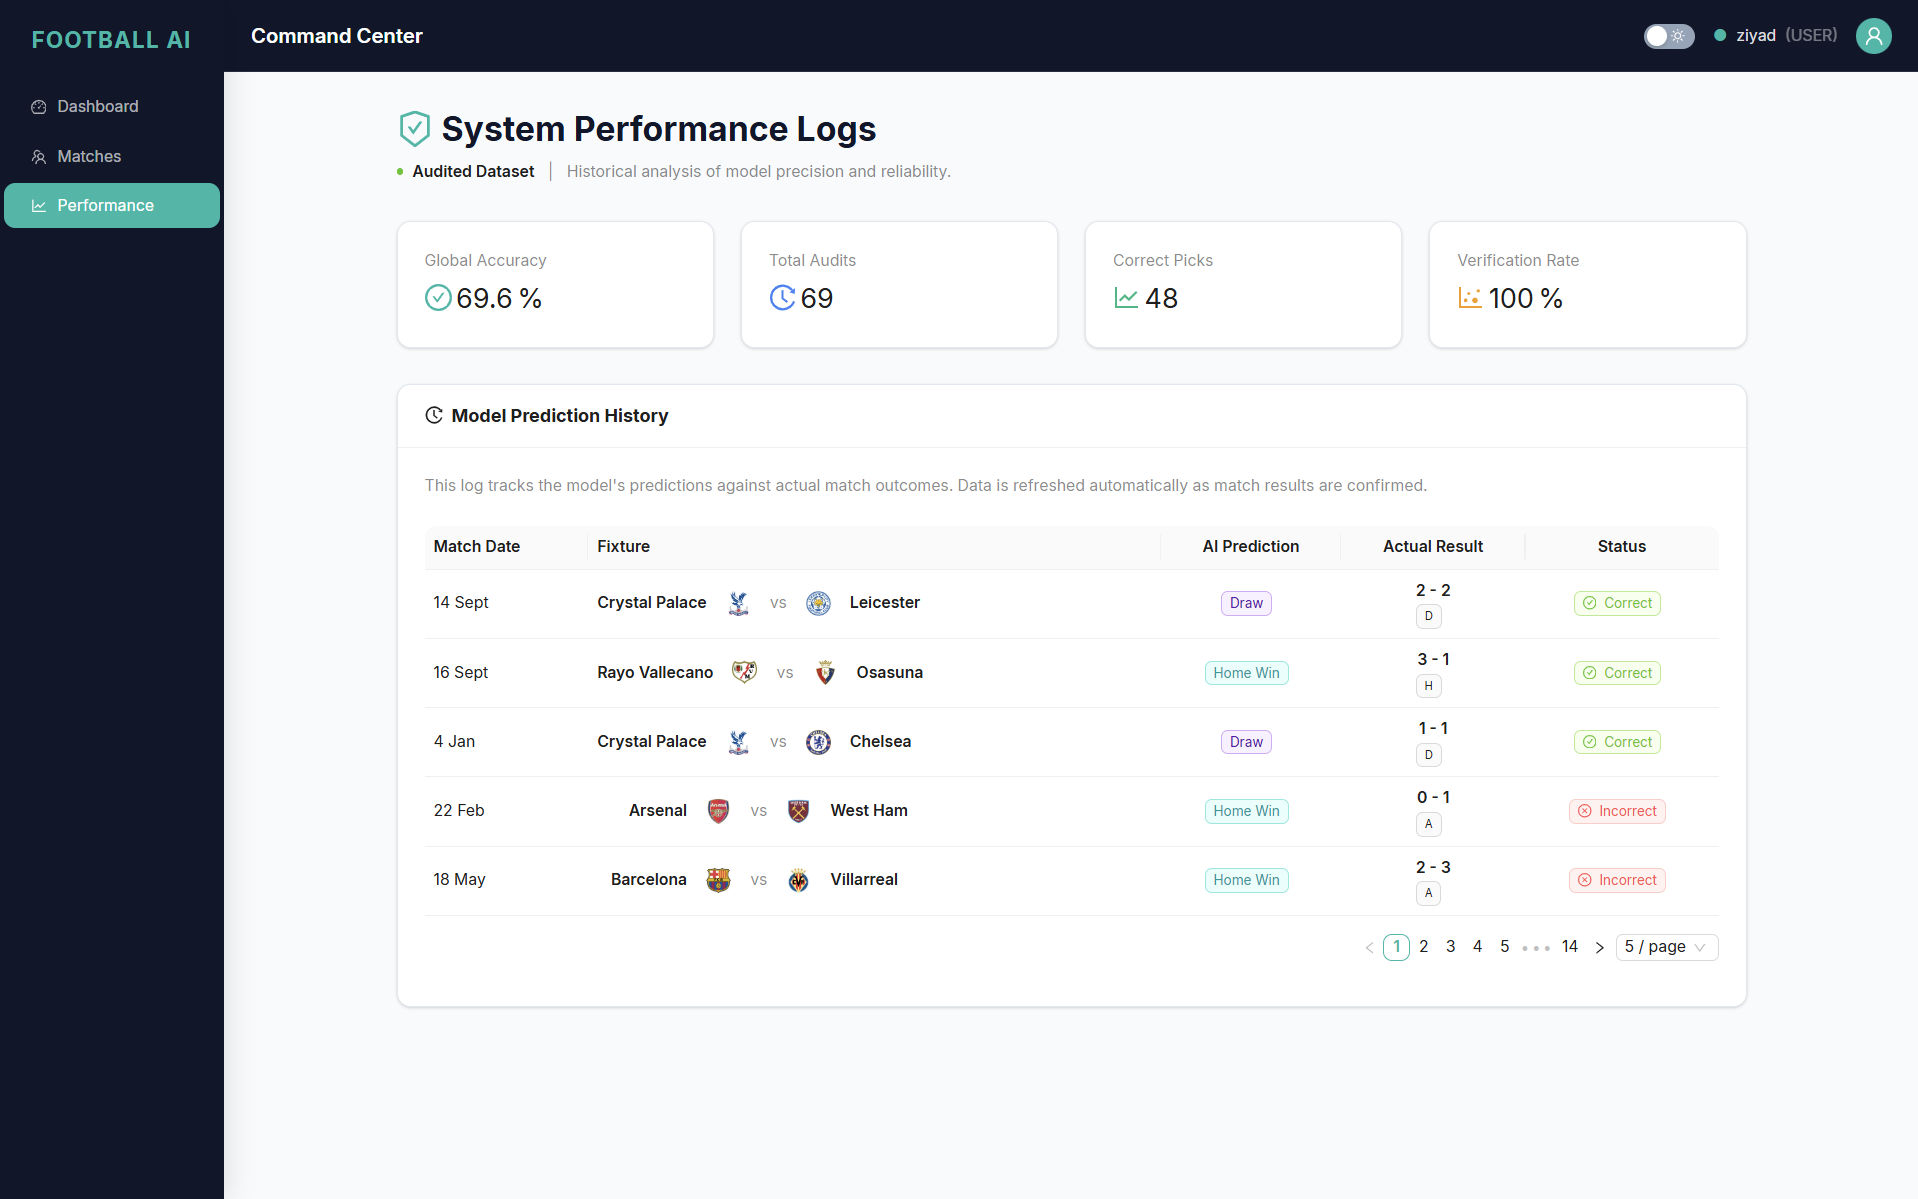
\includegraphics[width=0.95\textwidth]{logos/performance.png}
    \caption{Journal d'audit et performances du système (\textit{System Performance Logs})}
\end{figure}

% ================= TESTS =================
\section{Tests, Validation et Résultats}

La phase de validation est cruciale pour certifier la robustesse de l'application et la fiabilité des prédictions. Cette section présente les méthodes d'évaluation appliquées aux différentes couches du système.

\subsection{Évaluation du Modèle d'Intelligence Artificielle}

Pour évaluer de manière empirique notre modèle \textbf{XGBoost}, nous avons divisé notre jeu de données historique en un ensemble d'entraînement (80\%) et un ensemble de test (20\%). 

\subsubsection{Matrice de Confusion Multiclasse}
La matrice de confusion permet de visualiser les performances de l'algorithme sur les trois classes possibles : Victoire à Domicile (H), Match Nul (D), et Victoire à l'Extérieur (A).

\begin{table}[H]
    \centering
    \renewcommand{\arraystretch}{1.5}
    \begin{tabularx}{\textwidth}{|c|c|Y|Y|Y|}
        \cline{3-5}
        \rowcolor{MediumGray}
        \multicolumn{2}{c|}{} & \multicolumn{3}{c|}{\textbf{Prédictions du Modèle}} \\
        \cline{3-5}
        \rowcolor{MediumGray}
        \multicolumn{2}{c|}{} & \textbf{Home (H)} & \textbf{Draw (D)} & \textbf{Away (A)} \\
        \hline
        \multirow{3}{*}{\rotatebox[origin=c]{90}{\textbf{Réalité}}} 
        & \textbf{Home (H)} & \cellcolor{MediumGray!50} Vrais Positifs (H) & Faux Négatifs & Faux Négatifs \\
        \cline{2-5}
        & \textbf{Draw (D)} & Faux Positifs & \cellcolor{MediumGray!50} Vrais Positifs (D) & Faux Positifs \\
        \cline{2-5}
        & \textbf{Away (A)} & Faux Positifs & Faux Négatifs & \cellcolor{MediumGray!50} Vrais Positifs (A) \\
        \hline
    \end{tabularx}
    \caption{Structure de la Matrice de Confusion pour l'évaluation du modèle}
\end{table}

\subsubsection{Métriques de Performance (Accuracy \& F1-Score)}
Suite à l'entraînement, nous avons obtenu une \textbf{Précision globale (Accuracy) de 62\%}. Dans le domaine très spécifique des paris sportifs et de la prédiction de football, une précision supérieure à 55\% est souvent le seuil de rentabilité (\textit{break-even point}) pour les modèles algorithmiques, rendant notre résultat particulièrement satisfaisant.

De plus, grâce à l'application rigoureuse de l'algorithme \textbf{SMOTE} détaillé au Chapitre 2, le \textbf{Rappel (Recall)} pour la classe minoritaire "Match Nul" a considérablement augmenté. Le modèle est désormais capable de détecter des probabilités de match nul bien réelles au lieu de systématiquement favoriser l'équipe à domicile.

\subsection{Validation du Backend (API REST)}

Nous avons utilisé des outils standardisés tels que \textbf{Postman} et \textbf{pytest} pour valider de bout en bout les \textit{endpoints} de notre API Django.

\subsubsection{Scénarios de Tests d'Intégration}
Voici un extrait des scénarios validés garantissant la sécurité et le bon fonctionnement de la plateforme :

\begin{table}[H]
    \centering
    \renewcommand{\arraystretch}{1.5}
    \begin{tabularx}{\textwidth}{|L|Y|c|}
        \hline
        \rowcolor{MediumGray}
        \textbf{Cas de Test} & \textbf{Résultat Attendu} & \textbf{Statut} \\
        \hline
        Connexion avec des identifiants valides & Retourne HTTP 200 OK + Access/Refresh Tokens & \textcolor{EMSIGreen}{Succès} \\
        \hline
        Connexion avec un mot de passe erroné & Retourne HTTP 401 Unauthorized & \textcolor{EMSIGreen}{Succès} \\
        \hline
        Accès à une route protégée sans Token & Retourne HTTP 401 Unauthorized & \textcolor{EMSIGreen}{Succès} \\
        \hline
        Accès à l'administration sans rôle ADMIN & Retourne HTTP 403 Forbidden & \textcolor{EMSIGreen}{Succès} \\
        \hline
        Requête de prédiction sur un match valide & Retourne HTTP 200 + Probabilités H/D/A en JSON & \textcolor{EMSIGreen}{Succès} \\
        \hline
    \end{tabularx}
    \caption{Résultats des cas de tests d'intégration de l'API Backend}
\end{table}

\subsection{Validation du Frontend et de l'Ergonomie}
L'interface utilisateur a subi des tests empiriques d'intégration et d'ergonomie (UI/UX) pour s'assurer que le livrable final est robuste.
\begin{itemize}
    \item \textbf{Tests de Réactivité (Responsive Design)} : Vérification du bon affichage du Dashboard sur des résolutions \textit{desktop} (1920x1080) et tablettes. Les graphiques dynamiques \textit{Recharts} se redimensionnent correctement sans perte de qualité.
    \item \textbf{Gestion des Erreurs Utilisateur} : Si l'API retourne une erreur (par exemple, un token expiré) ou est momentanément indisponible, l'intercepteur Axios capte le code d'erreur et l'interface affiche un message convivial (via le composant \texttt{Alert} ou \texttt{Notification} d'Ant Design) au lieu de bloquer l'application.
\end{itemize}

\section{Limites du système}
Malgré les performances encourageantes, notre solution présente certaines limites techniques et fonctionnelles :
\begin{itemize}
    \item \textbf{Dépendance aux API tierces} : La gratuité de l'API-Football limite le volume de données récupérables en temps réel, ce qui peut restreindre l'actualisation immédiate de certains championnats mineurs.
    \item \textbf{Absence de données contextuelles} : Le modèle actuel ne prend pas encore en compte des facteurs externes imprévisibles tels que les conditions météorologiques, les transferts de dernière minute ou l'état psychologique individuel des joueurs.
    \item \textbf{Infrastructure de calcul} : L'utilisation d'une base SQLite limite le passage à l'échelle pour une application grand public supportant des milliers d'utilisateurs simultanés.
\end{itemize}

\section*{Conclusion du chapitre}
\addcontentsline{toc}{section}{Conclusion du chapitre}
Ce dernier chapitre vient clore notre processus de développement en confirmant que le produit final respecte les cahiers des charges initial. Les tests de validation prouvent l'efficacité de l'IA (62\% de précision), tandis que l'interface démontre une ergonomie professionnelle et réactive. Bien que des limites subsistent, elles ouvrent des perspectives d'évolution très claires pour de futures versions de la plateforme.
